\documentclass[11pt,a4paper]{book}
\usepackage[margin=2in]{geometry}
\usepackage[italian]{babel}
\usepackage[T1]{fontenc}
\usepackage[utf8]{inputenc}
\usepackage{graphicx}
\usepackage{imakeidx}
\usepackage{amsmath}
\usepackage[hyperfootnotes=false, colorlinks=true, linkcolor=black]{hyperref}
\usepackage[style=numeric-comp,useprefix,hyperref,backend=bibtex]{biblatex}
\usepackage{listings}  % Serve per evidenziare i blocchi di codice
\usepackage{pxfonts} % permette di avere caratteri in lstlisting con formattazione

\setlength{\parskip}{1em} % cambia l'interlinea prima di un nuovo capoverso

\usepackage{xcolor} % Necessario per definire i colori
\hypersetup{
  colorlinks=true,
  linkcolor=green!70!black,
  urlcolor=green!70!black
} % Setup colore link

\begin{document}
\title{MongoDB - Udemy}
\author{Jacopo De Angelis}
\maketitle

\pagebreak
\tableofcontents
\pagebreak

\chapter{Perchè un database noSQL?}
I database noSQL nascono per esigenze particolari con tre obiettivi principali:
\begin{itemize}
	\item scalabilità: un sistema più comodo per i big data 
	\item facilità dello sviluppo
	\item rappresentazione intuitiva: dati semi-strutturati, non strutturati, strutture dati complesse, polimorfismo
\end{itemize}

Scalabilità:
\begin{itemize}
	\item verticale: potenziamento della macchina singola
	\item orizzontale: moltiplicazione delle macchine a disposizione
\end{itemize}
Per quanto molto vantaggiosa, la scalabilità orizzontale porta il problema di passaggio delle informazioni tra i vari server.
\begin{figure}[h!]
	\begin{center}
		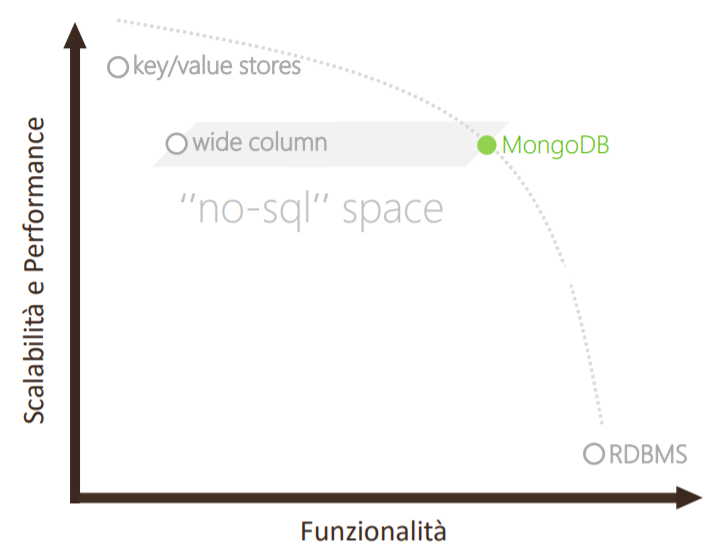
\includegraphics[scale=0.6]{img/001.png}
		\caption{Rapporto funzionalità/scalabilità}
		\label{fig: 001}
	\end{center}
\end{figure}
MongoDB rinuncia a joins e transactions.

\chapter{Funzionalità}
\section{Join e transactions}
Ha rinunciato a queste due funzioni in nome della scalabilità, infatti come si poterebbero ottimizzare le performance su più server?
\begin{itemize}
	\item[] Copiando le tabelle ovunque? Non sarebbe vera scalabilità
	\item[] Dividendole su più server? Auguri nel caso si voglia accedere ad una tabella di join su più server
\end{itemize}
Si usa l'approccio "document-oriented", ovvero un'intuitiva rappresentazione dei dati (in questo caso i documenti sono uguali agli oggetti della programmazione orientata agli oggetti, sono contenitori di informazioni). Si usa quindi la codifica JSON\footnote{JavaScript Object Notation}.

Per risolvere il problema delle join e transactions si usano le \textbf{pre-join e l'embedding}. Le pre-join sono il contrario delle join, ovvero si usano dati che contengono tutte le informazioni e da queste le scorporiamo all'occorrenza. Ovvero la tabella avrà una struttura piatta, dove in ogni oggetto verranno inclusi tutti i dati che avremmo normalmente in una join.
\begin{figure}[h!]
	\begin{center}
		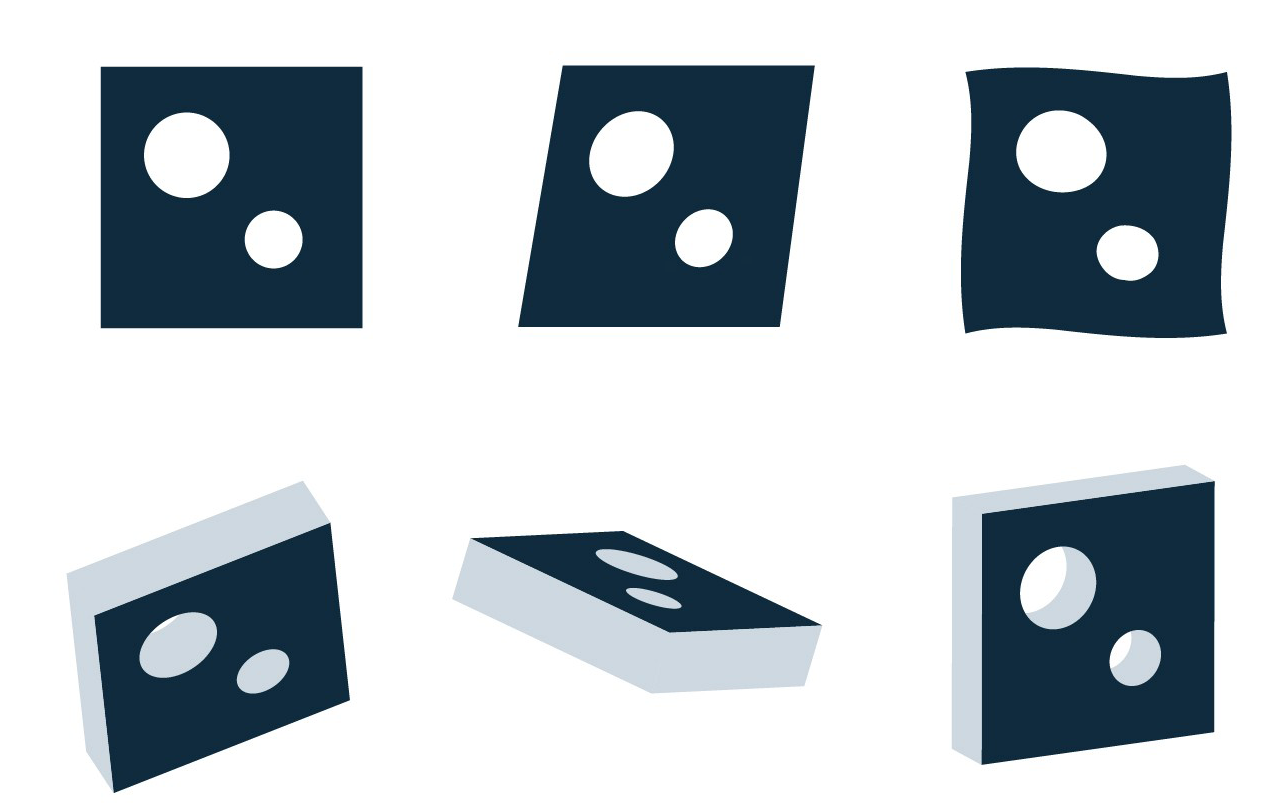
\includegraphics[scale=0.6]{img/008.png}
		\caption{Differenza tra relazionale e noSQL}
		\label{fig: 008}
	\end{center}
\end{figure}

\paragraph{Schemaless} 
MongoDB è schemaless, ovvero non ha schema statico e se volessimo aggiungere altri attributi ci basterebbe aggiungerli nel documento.

\paragraph{Replication e auto-sharding}
Fanno parte della scalabilità.

\textbf{Replication}: copia e sincronizzazione dei dati tra i vari server

\textbf{Sharding}: permette di separare i dati su più server e MongoDB si occuperà di gestire i carichi

\begin{figure}[h!]
	\begin{center}
		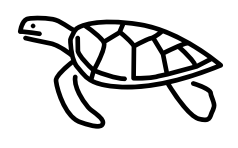
\includegraphics[scale=0.6]{img/009.png}
		\caption{Nuova terminologia}
		\label{fig: 009}
	\end{center}
\end{figure}
 


\subsection{JSON}
Un oggetto è una serie non ordinata di nomi/valori. Un oggetto inizia con {parentesi graffa sinistra e finisce con }parentesi graffa destra. Ogni nome è seguito da :due punti e la coppia di nome/valore sono separata da ,virgola.
\begin{figure}[h!]
	\begin{center}
		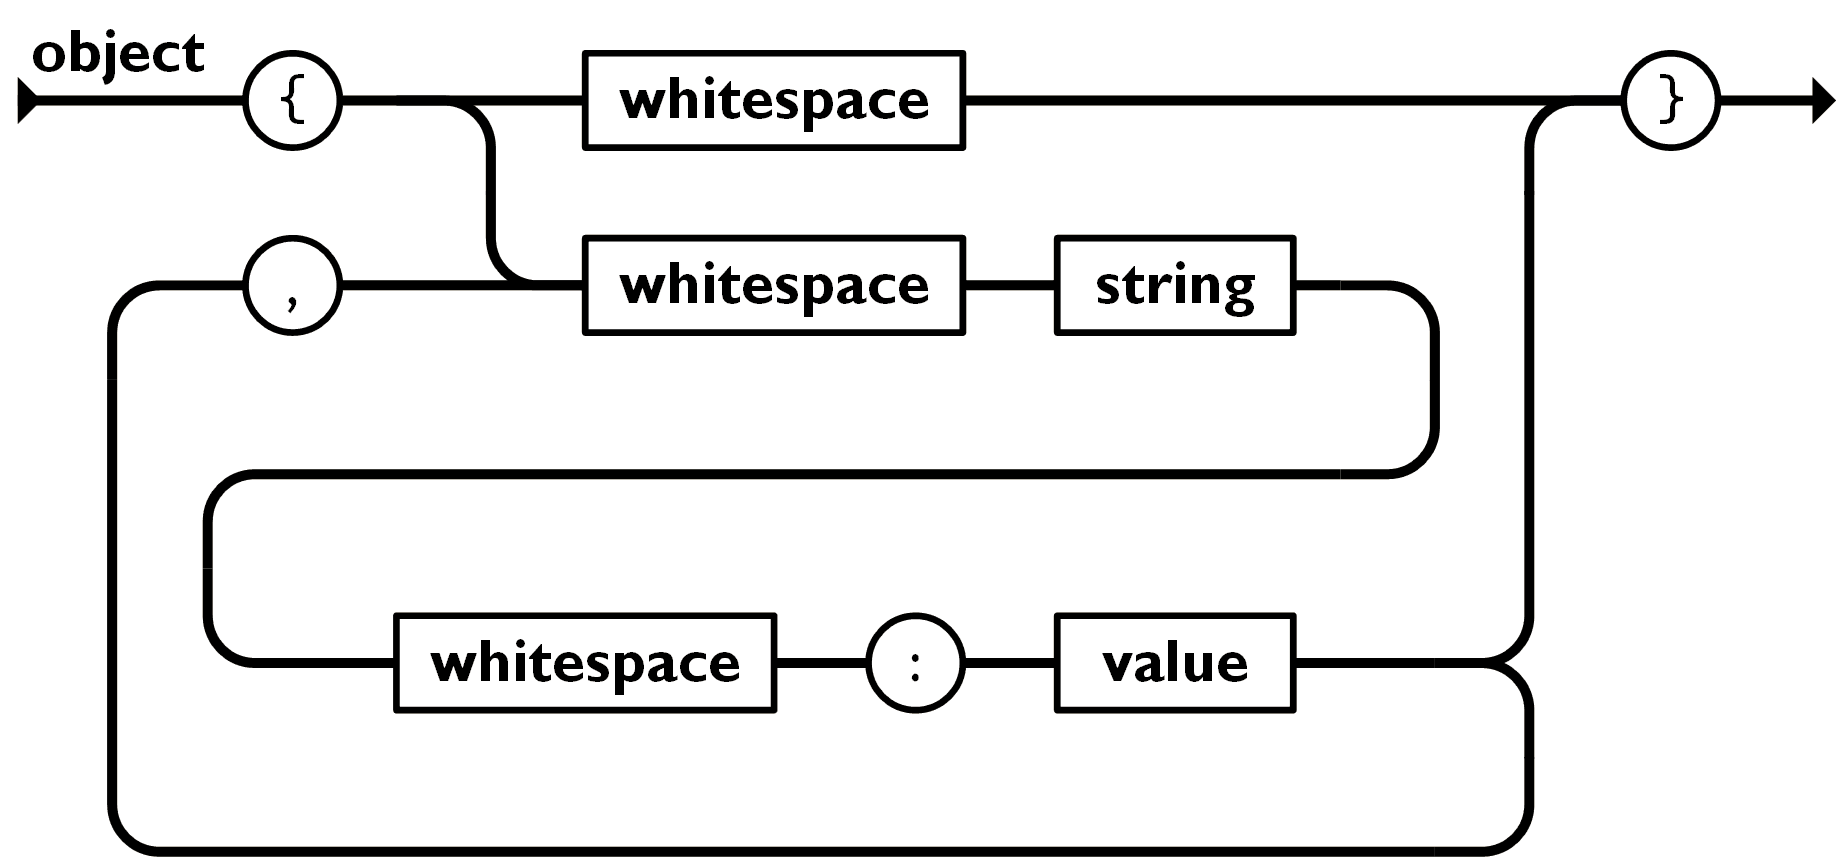
\includegraphics[scale=0.6]{img/002.png}
		\caption{JSON: parser oggetto}
		\label{fig: 002}
	\end{center}
\end{figure}

\clearpage
Un array è una raccolta ordinata di valori. Un array comincia con [parentesi quadra sinistra e finisce con ]parentesi quadra destra. I valori sono separati da ,virgola.
\begin{figure}[h!]
	\begin{center}
		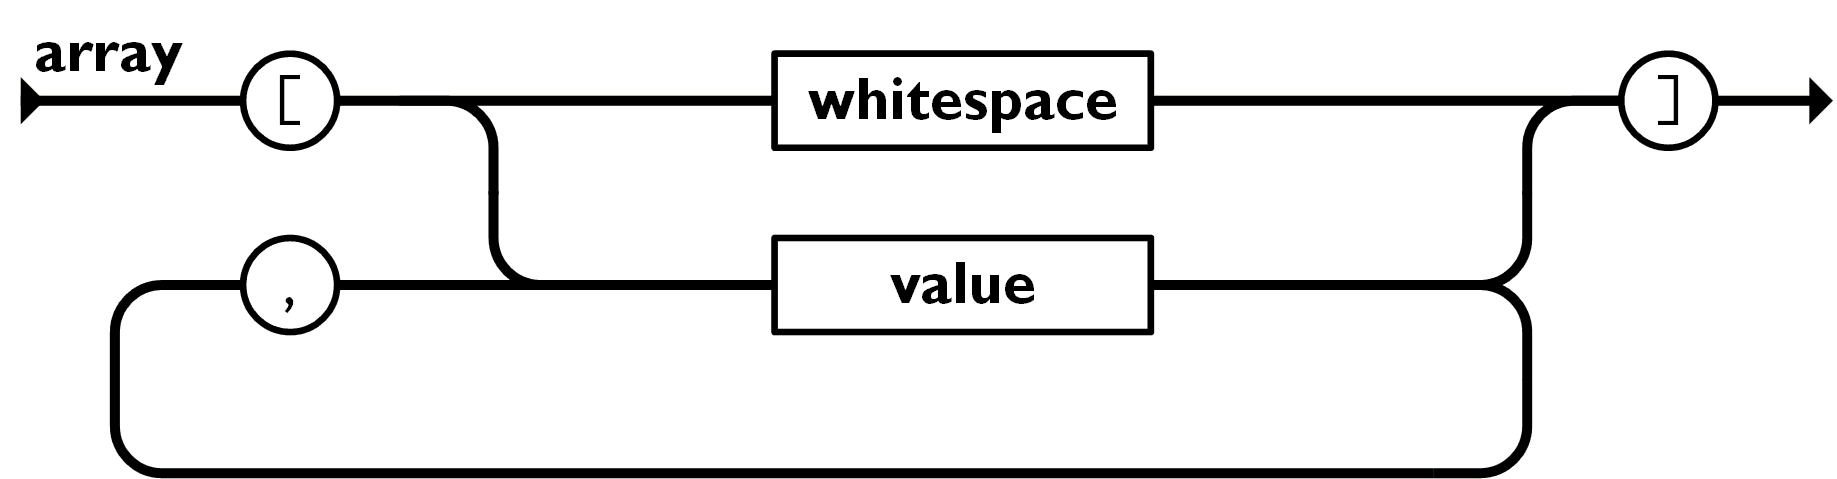
\includegraphics[scale=0.6]{img/003.png}
		\caption{JSON: parser array}
		\label{fig: 003}
	\end{center}
\end{figure}

\clearpage
Un valore può essere una stringa tra virgolette, o un numero, o vero true o falso false o nullo null, o un oggetto o un array. Queste strutture possono essere annidate.
\begin{figure}[h!]
	\begin{center}
		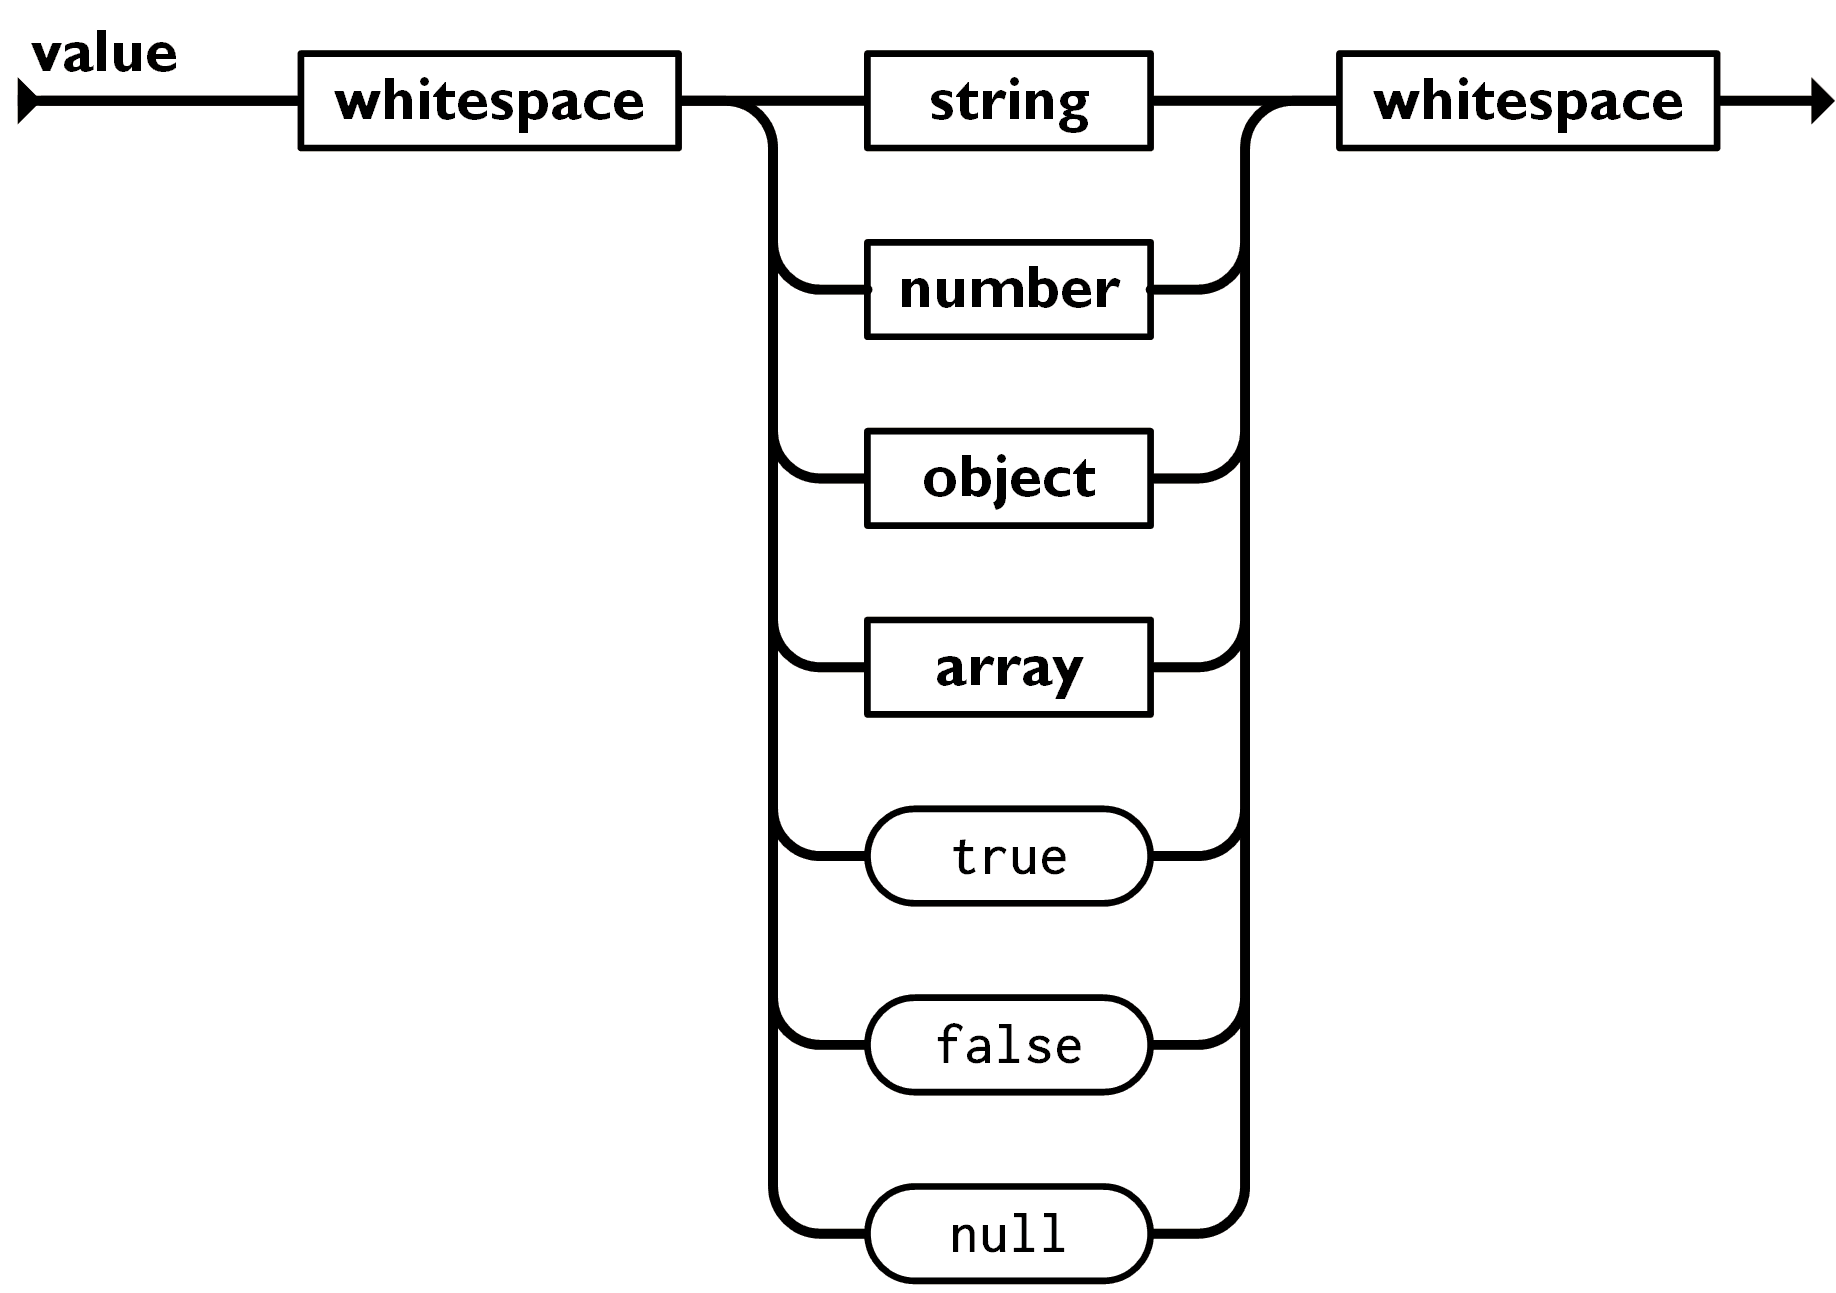
\includegraphics[scale=0.6]{img/004.png}
		\caption{JSON: parser valore}
		\label{fig: 004}
	\end{center}
\end{figure}

\clearpage
Una stringa è una raccolta di zero o più caratteri Unicode, tra virgolette; per le sequenze di escape utilizza la barra rovesciata. Un singolo carattere è rappresentato come una stringa di caratteri di lunghezza uno. Una stringa è molto simile ad una stringa C o Java.
\begin{figure}[h!]
	\begin{center}
		
\includegraphics[scale=0.6]{img/005.png}
		\caption{JSON: parser stringa}
		\label{fig: 005}
	\end{center}
\end{figure}

\clearpage
Un numero è molto simile ad un numero C o Java, a parte il fatto che i formati ottali e esadecimali non sono utilizzati.
\begin{figure}[h!]
	\begin{center}
		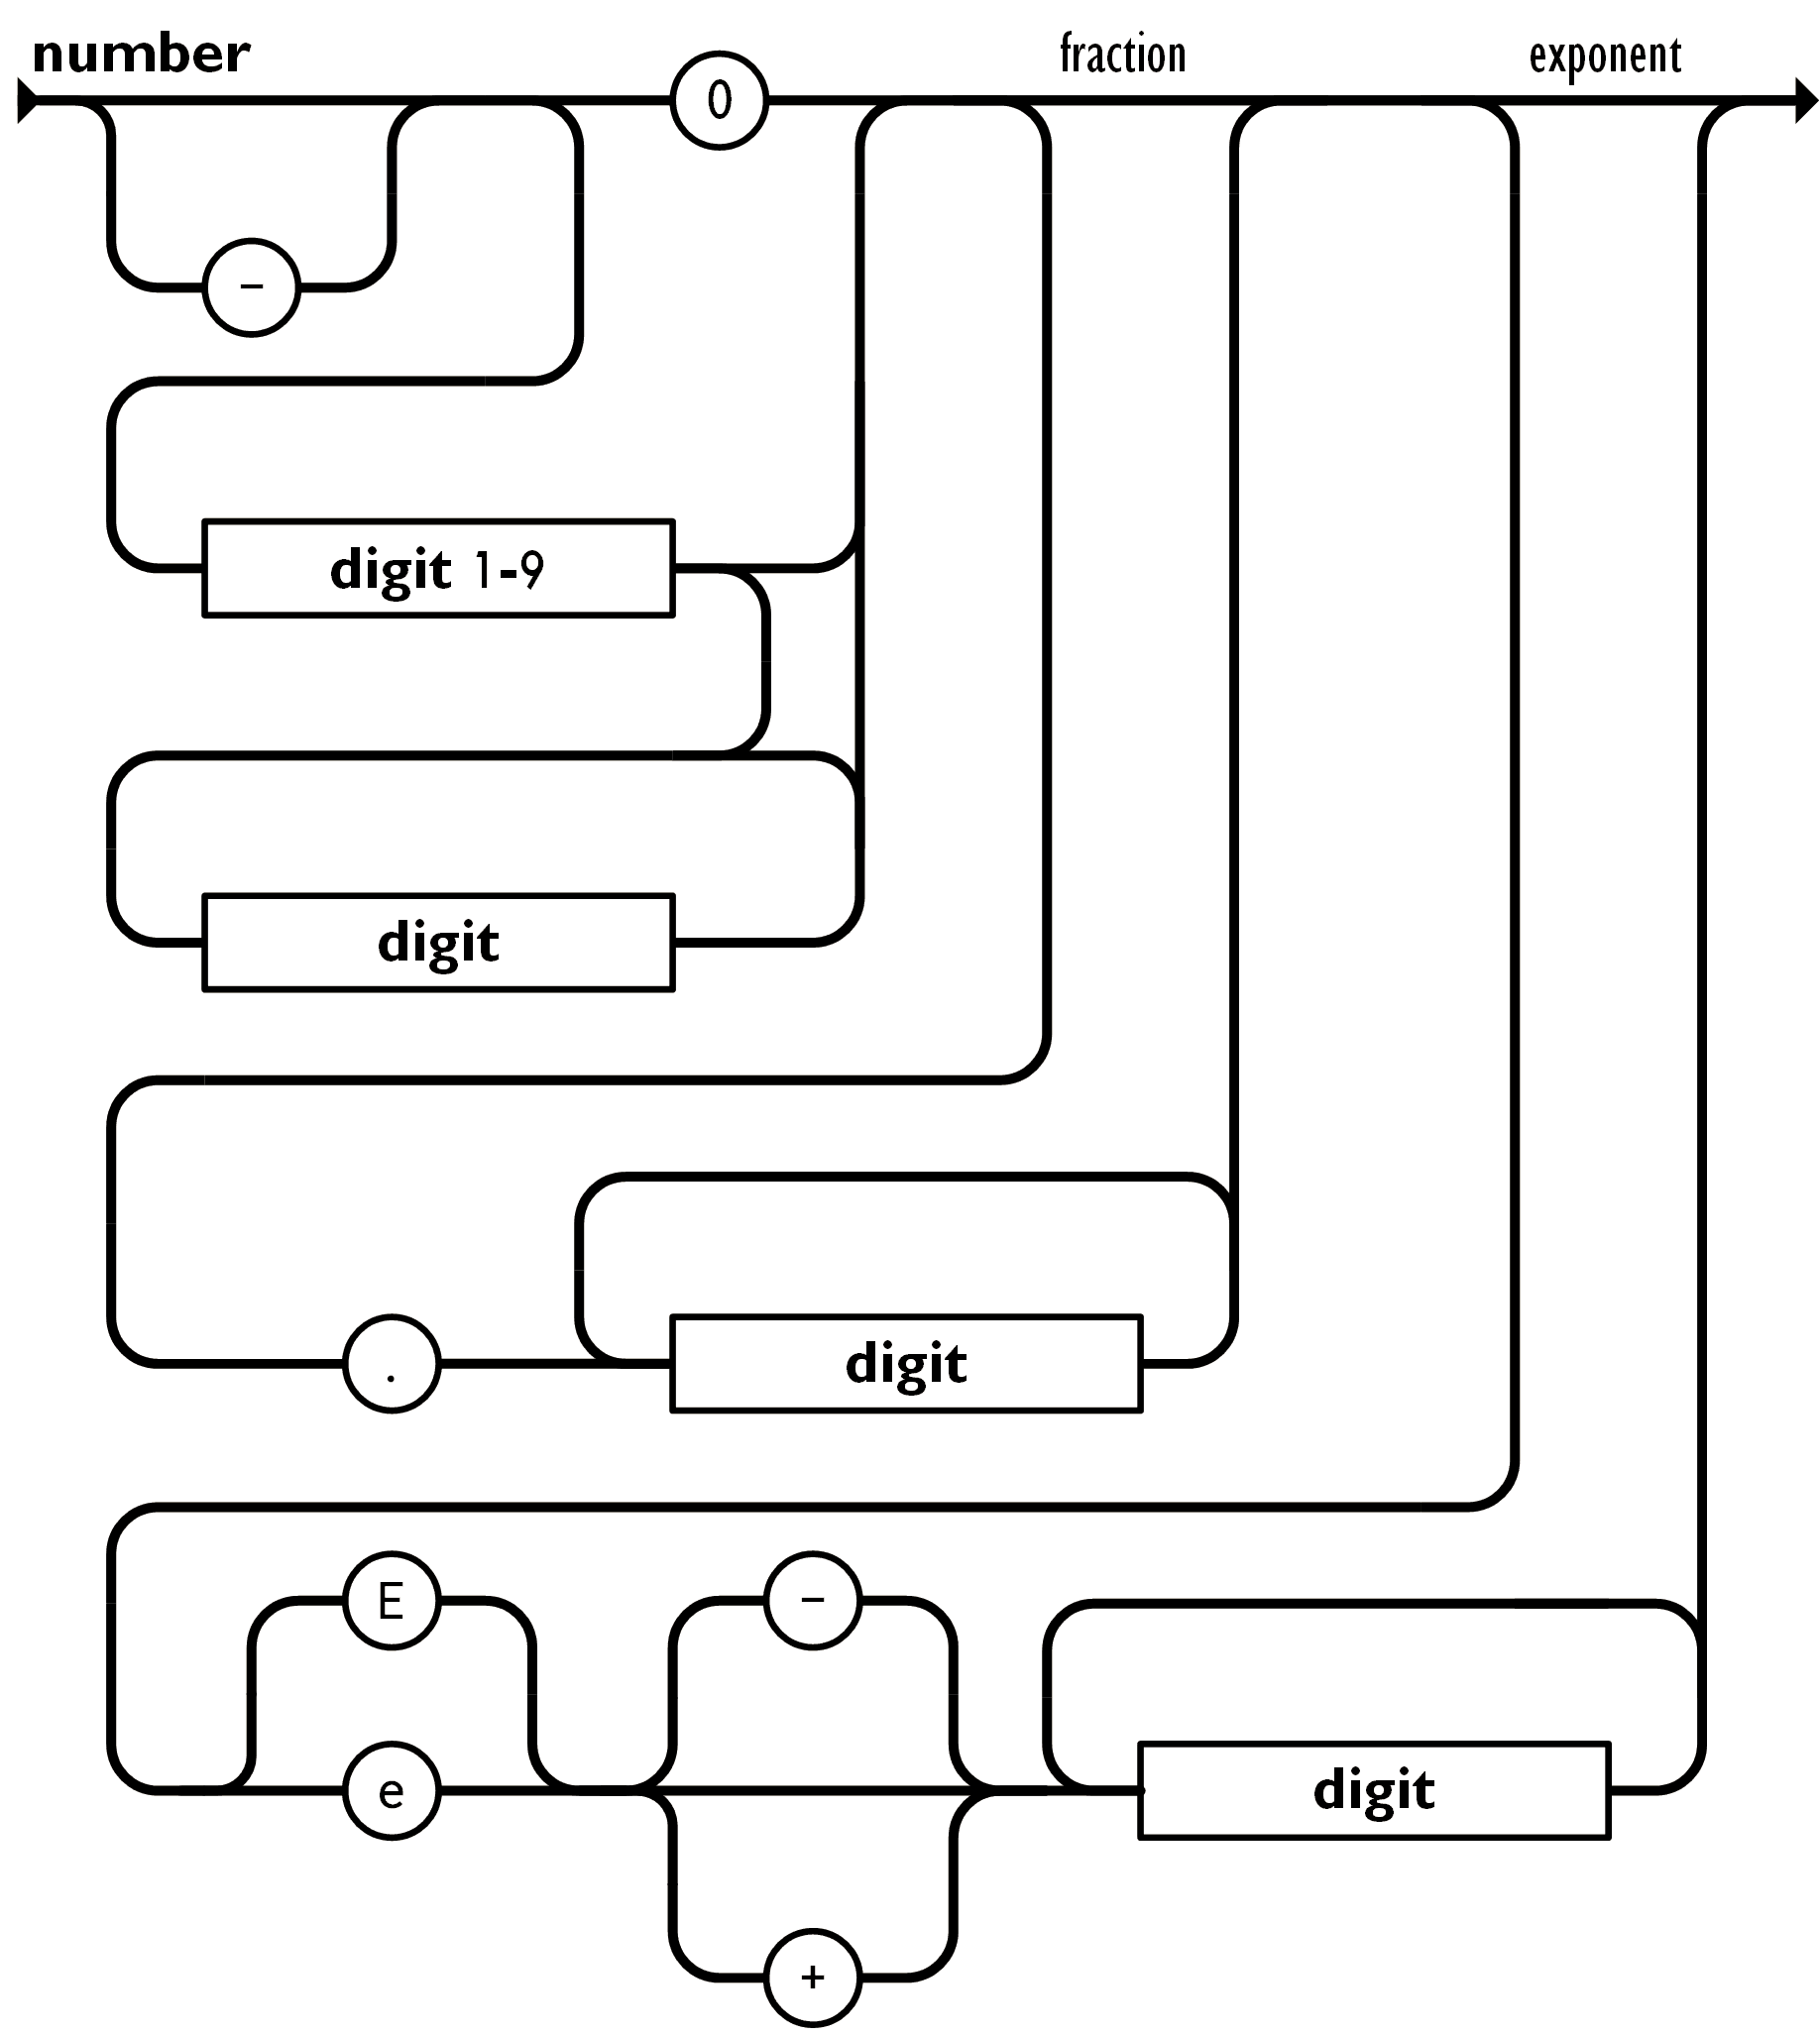
\includegraphics[scale=0.6]{img/006.png}
		\caption{JSON: parser numero}
		\label{fig: 006}
	\end{center}
\end{figure}

\clearpage
I caratteri di spaziatura possono essere inseriti in mezzo a qualsiasi coppia di token. A parte alcuni dettagli di codifica, questo descrive totalmente il linguaggio.
\begin{figure}[h!]
	\begin{center}
		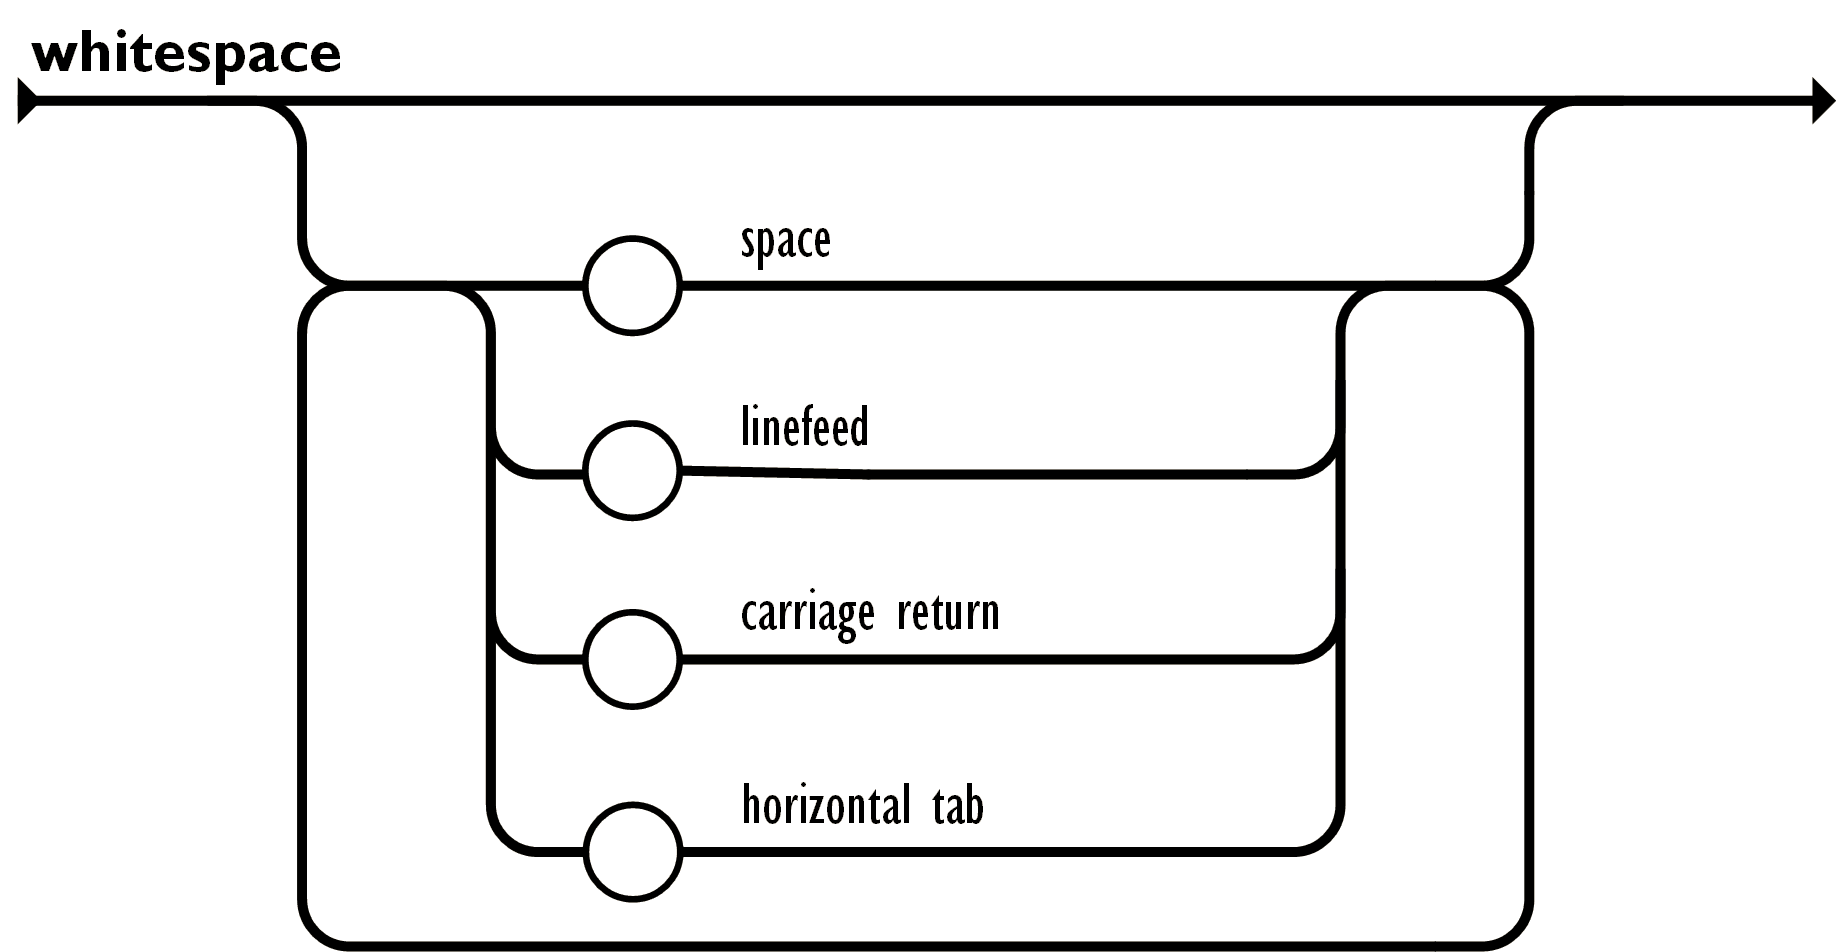
\includegraphics[scale=0.6]{img/007.png}
		\caption{JSON: parser spaziatura}
		\label{fig: 007}
	\end{center}
\end{figure}
\clearpage

\textbf{Esempio di oggetto JSON}:
\begin{lstlisting}[language = ]
{"menu": {
    "header": "SVG Viewer",
    "items": [
        {"id": "Open"},
        {"id": "OpenNew", "label": "Open New"},
        null,
        {"id": "ZoomIn", "label": "Zoom In"},
        {"id": "ZoomOut", "label": "Zoom Out"},
        {"id": "OriginalView", "label": "Original View"},
        null,
        {"id": "Quality"},
        {"id": "Pause"},
        {"id": "Mute"},
        null,
        {"id": "Find", "label": "Find..."},
        {"id": "FindAgain", "label": "Find Again"},
        {"id": "Copy"},
        {"id": "CopyAgain", "label": "Copy Again"},
        {"id": "CopySVG", "label": "Copy SVG"},
        {"id": "ViewSVG", "label": "View SVG"},
        {"id": "ViewSource", "label": "View Source"},
        {"id": "SaveAs", "label": "Save As"},
        null,
        {"id": "Help"},
        {"id": "About", "label": "About Adobe CVG Viewer..."}
    ]
}}
\end{lstlisting}

\section{MongoDB in un'app}
Nell'applicazione, scritta nel linguaggio preferita, avremo richieste dai vari utenti. In un'app classica avremo anche un database con i vari dati. Per connettere app e database avremo bisogno di un driver, scaricabile dal sito.

Quando l'app richiede al database i dati, questi vengono spediti in BSON, ovvero il formato binario del JSON e poi, grazie al connettore (il driver) verranno convertiti nella struttura dati base del linguaggio.

\end{document}